\documentclass[journal,12pt,twocolumn]{IEEEtran}

\usepackage{setspace}
\usepackage{gensymb}
\singlespacing
\usepackage{amsmath}
\usepackage{amsthm}

\usepackage{mathrsfs}
\usepackage{txfonts}
\usepackage{stfloats}
\usepackage{bm}
\usepackage{cite}
\usepackage{cases}
\usepackage{subfig}

\usepackage{longtable}
\usepackage{multirow}

\usepackage{enumitem}
\usepackage{mathtools}
\usepackage{steinmetz}
\usepackage{tikz}
\usepackage{circuitikz}
\usepackage{verbatim}
\usepackage{tfrupee}
\usepackage[breaklinks=true]{hyperref}
\usepackage{graphicx}
\usepackage{tkz-euclide}

\usetikzlibrary{calc,math}
\usepackage{listings}
    \usepackage{color}                                            %%
    \usepackage{array}                                            %%
    \usepackage{longtable}                                        %%
    \usepackage{calc}                                             %%
    \usepackage{multirow}                                         %%
    \usepackage{hhline}                                           %%
    \usepackage{ifthen}                                           %%
    \usepackage{lscape}     
\usepackage{multicol}
\usepackage{chngcntr}

\DeclareMathOperator*{\Res}{Res}

\renewcommand\thesection{\arabic{section}}
\renewcommand\thesubsection{\thesection.\arabic{subsection}}
\renewcommand\thesubsubsection{\thesubsection.\arabic{subsubsection}}

\renewcommand\thesectiondis{\arabic{section}}
\renewcommand\thesubsectiondis{\thesectiondis.\arabic{subsection}}
\renewcommand\thesubsubsectiondis{\thesubsectiondis.\arabic{subsubsection}}


\hyphenation{op-tical net-works semi-conduc-tor}
\def\inputGnumericTable{}                                 %%

\lstset{
%language=C,
frame=single, 
breaklines=true,
columns=fullflexible
}

\begin{document}

\newcommand{\BEQA}{\begin{eqnarray}}
\newcommand{\EEQA}{\end{eqnarray}}
\newcommand{\define}{\stackrel{\triangle}{=}}
\bibliographystyle{IEEEtran}
\raggedbottom
\setlength{\parindent}{0pt}
\providecommand{\mbf}{\mathbf}
\providecommand{\pr}[1]{\ensuremath{\Pr\left(#1\right)}}
\providecommand{\qfunc}[1]{\ensuremath{Q\left(#1\right)}}
\providecommand{\sbrak}[1]{\ensuremath{{}\left[#1\right]}}
\providecommand{\lsbrak}[1]{\ensuremath{{}\left[#1\right.}}
\providecommand{\rsbrak}[1]{\ensuremath{{}\left.#1\right]}}
\providecommand{\brak}[1]{\ensuremath{\left(#1\right)}}
\providecommand{\lbrak}[1]{\ensuremath{\left(#1\right.}}
\providecommand{\rbrak}[1]{\ensuremath{\left.#1\right)}}
\providecommand{\cbrak}[1]{\ensuremath{\left\{#1\right\}}}
\providecommand{\lcbrak}[1]{\ensuremath{\left\{#1\right.}}
\providecommand{\rcbrak}[1]{\ensuremath{\left.#1\right\}}}
\theoremstyle{remark}
\newtheorem{rem}{Remark}
\newcommand{\sgn}{\mathop{\mathrm{sgn}}}
\providecommand{\abs}[1]{\vert#1\vert}
\providecommand{\res}[1]{\Res\displaylimits_{#1}} 
\providecommand{\norm}[1]{\lVert#1\rVert}
%\providecommand{\norm}[1]{\lVert#1\rVert}
\providecommand{\mtx}[1]{\mathbf{#1}}
\providecommand{\mean}[1]{E[ #1 ]}
\providecommand{\fourier}{\overset{\mathcal{F}}{ \rightleftharpoons}}
%\providecommand{\hilbert}{\overset{\mathcal{H}}{ \rightleftharpoons}}
\providecommand{\system}{\overset{\mathcal{H}}{ \longleftrightarrow}}
	%\newcommand{\solution}[2]{\textbf{Solution:}{#1}}
\newcommand{\solution}{\noindent \textbf{Solution: }}
\newcommand{\cosec}{\,\text{cosec}\,}
\providecommand{\dec}[2]{\ensuremath{\overset{#1}{\underset{#2}{\gtrless}}}}
\newcommand{\myvec}[1]{\ensuremath{\begin{pmatrix}#1\end{pmatrix}}}
\newcommand{\mydet}[1]{\ensuremath{\begin{vmatrix}#1\end{vmatrix}}}
\numberwithin{equation}{subsection}
\makeatletter
\@addtoreset{figure}{problem}
\makeatother
\let\StandardTheFigure\thefigure
\let\vec\mathbf
\renewcommand{\thefigure}{\theproblem}
\def\putbox#1#2#3{\makebox[0in][l]{\makebox[#1][l]{}\raisebox{\baselineskip}[0in][0in]{\raisebox{#2}[0in][0in]{#3}}}}
     \def\rightbox#1{\makebox[0in][r]{#1}}
     \def\centbox#1{\makebox[0in]{#1}}
     \def\topbox#1{\raisebox{-\baselineskip}[0in][0in]{#1}}
     \def\midbox#1{\raisebox{-0.5\baselineskip}[0in][0in]{#1}}
\vspace{3cm}
\title{Assignment 5- Probability and Random Variables}
\author{Songa Kotesh Satvik}
\maketitle
\newpage
\bigskip
\renewcommand{\thefigure}{\theenumi}
\renewcommand{\thetable}{\theenumi}
Download all python codes from 
\begin{lstlisting}
https://github.com/KoteshSatvik/AI1103-Probability_and_Random_Variables/tree/main/Assignment-5/codes
\end{lstlisting}
%
and latex-tikz codes from 
%
\begin{lstlisting}
https://github.com/KoteshSatvik/AI1103-Probability_and_Random_Variables/blob/main/Assignment-5/Assignment5.tex
\end{lstlisting}
\section{\textbf{Gate 2015 (ee paper-1 new 2) Q.2(apt. section)}}
Given Set A = \{2,3,4,5\} and Set B = \{11,12,13,14,15\}, two numbers are randomly selected, one from each set. What is probability that the sum of the two numbers equals 16?
\section{\textbf{Solution}}
Let $X_1\in\,$\cbrak{2,3,4,5} and $X_2\in\,$\cbrak{11,12,13,14,15} be the random variables such that $X_1$ represents the number chosen from set A and $X_2$ the number chosen from set B.\\
Then, the probability mass functions are 
\begin{align}
    p_{X_1}(n) = \pr{X_1 = n} = 
    \begin{cases}
    \frac{1}{4} & 2 \leq n \leq 5\\
    0 & otherwise
\end{cases}\label{1}
\end{align}
\begin{align}
    p_{X_2}(n) = \pr{X_2 = n} = 
    \begin{cases}
    \frac{1}{5} & 11 \leq n \leq 15\\
    0 & otherwise
\end{cases}\label{2}
\end{align}
Let X be the random variable denoting the sum (X=$X_1$+$X_2$). Then, X can take the values \cbrak{13,14,15,16,17,18,19,20}.
\begin{align}
     p_X(n)&=\pr{X_1+X_2=n}\\
     &=\pr{X_1=n-X_2}\\
     &=\Sigma_{k}{\pr{X_1=n-k|X_2=k}p_{X_2}(k)}\label{3}
\end{align}
 As $X_1,X_2$ are independent,
\begin{align}
    \pr{X_1=n-k|X_2=k}=\pr{X_1=n-k}\label{4}
\end{align}
from \eqref{3} and \eqref{4}
\begin{align}
    p_X(n) = \Sigma_{k} p_{X_1}(n-k)p_{X_2}(n)
    &= p_{X_1}(n)*p_{X_2}(n)\label{5}
\end{align}
where * denotes the convolution operator.\\
As,
\begin{align}
    p_X(n) &= \Sigma_{k} p_{X_1}(n-k)p_{X_2}(k)\\
    &= \frac{1}{5} \sum_{k=11}^{15}p_{X_1}(n-k)\\
    &= \frac{1}{5} \sum_{k=n-15}^{n-11} p_{X_1}(k)
\end{align}
Since $p_{X_1}(k)=0$ for $k<2 , k>5$\\
Therefore, we get 
\begin{align}
    p_x(n) = 
    \begin{cases}
    0 & n \leq 12\\
    \frac{1}{5} \sum_{k=2}^{n-11}p_{X_1}(k) & 2 \leq n-11 \leq 5\\
    \frac{1}{5} \sum_{k=n-15}^{5}p_{X_1}(k) & 2 \leq n-15 \leq 5\\
    0 & n>20
    \end{cases}
\end{align}
Therefore, from \eqref{1} we get
\begin{figure}[!hbt]
    \centering
    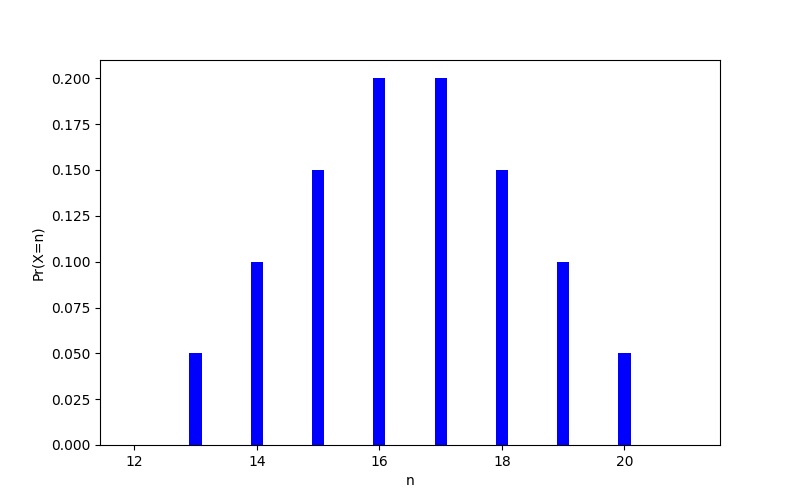
\includegraphics[width=\columnwidth]{Figure_1.png}
    \caption{Probability mass function of X}
    \label{Figure_1}
\end{figure}
\begin{align}
    p_x(n) = 
    \begin{cases}
    0 & n \leq 12\\
    \frac{n-12}{20}  & 13 \leq n \leq 16\\
    \frac{21-n}{20}  & 17 \leq n \leq 20\\
    0 & n>20
    \end{cases}\label{6}
\end{align}
Required probability is the probability of the sum of numbers selected from the sets, one from each set to be 16.\\
Therefore from \eqref{6},
\begin{align}
    p_X(16) &= \left(\frac{16-12}{20}\right)\\
    \implies p_X(16) &= \frac{4}{20}\\
    \implies\pr{X_1+X_2=16} &= \frac{1}{5} \\
    \therefore \pr{X_1+X_2=16}  &= 0.2
\end{align}
\end{document}